\documentclass[../memoria.tex]{subfiles}
\begin{document}
\label{marco teorico}

%AGREGAR CONTEXTO

\indent Un sistema típico de Re-ID tiene dos fases \cite{bedagkar2014survey}: (1) captura de descriptores y (2) comparación de descriptores, tal como se muestra en la figura \ref{fig:sistemaReID}. %se puede ver una representación esquemática de un sistema de Re-ID, mostrando las dos fases mencionadas anteriormente y los sub-procesos dentro de cada una.

\begin{figure}[h!]
  \centering
  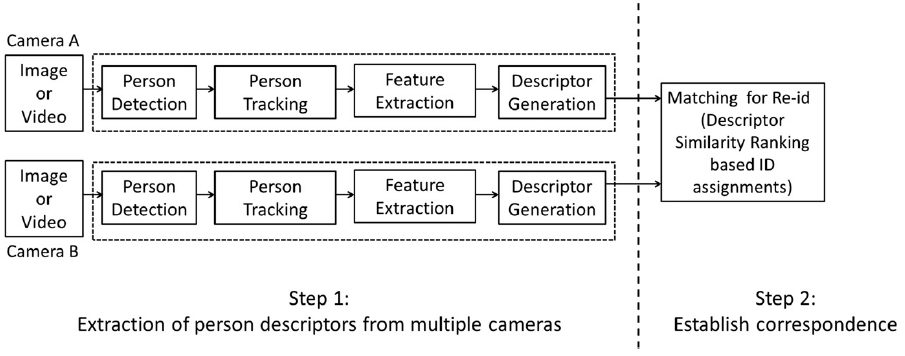
\includegraphics[width=\textwidth]{diagrama1.png}
  \caption{Sistema de Re-ID \cite{bedagkar2014survey}}
  \label{fig:sistemaReID}
\end{figure}

\indent En una primera fase, se extrae el descriptor de una persona desde múltiples cámaras (o en nuestro caso, distintas ocurrencias desde una misma cámara). En la segunda fase, se establece la correspondencia entre pares de descriptores, determinando si estos coinciden con la misma persona o son individuos distintos.

\indent Las tareas típicas de la primera fase incluyen \cite{yilmaz2006object}:
	\begin{itemize}
	\item \underline{Detección de personas:} se establece la presencia de personas en una escena. Para esto, se pueden utilizar algoritmos de aprendizaje supervisado cuando se cuenta con una base de datos con imágenes etiquetadas \cite{dalal2005histograms}. En el caso de un video, existen varias imágenes consecutivas (cuadros o \emph{frames}), lo que permite detectar cuando la persona se mueve o desplaza por la escena, según los cambios producidos en cada píxel. Esto se conoce como segmentación entre primer y segundo plano (que corresponden al movimiento y regiones estáticas, respectivamente).

	\indent La detección del segundo plano permite eliminar de la imagen todo lo que no forma parte de la persona, ocultando todo el conjunto de píxeles que permanezcan sin cambios. Para esto, se utiliza un mapa de bits o matriz de ceros y unos, que se superpone a la imagen original, convirtiendo el segundo plano en un mismo valor (bit cero: color negro), dejando los píxeles del primer plano inalterados (bit uno: color original) \cite{bouwmans2008background}. Luego, un algoritmo de detección de bordes \cite{canny1986computational} encuentra fronteras entre regiones similares, obteniendo la silueta del objeto o persona en movimiento. En algunas ocasiones, cuando existe alto grado de contraste entre una persona y el fondo (como en una toma a la misma altura del individuo) la detección de bordes puede prescindir de la segmentación. Sin embargo, ésta permite obtener bordes con menos posibilidad de error, dado que todo el fondo tiene un mismo valor \cite{bouwmans2008background}.

	%EXPLICAR "A QUÉ VIENE ESTO", TAL VEZ CONTEXTUALIZAR - REDACTAR DE NUEVO
	\indent Las formas detectadas, en la práctica no siempre se producen por un movimiento real de personas. También se detectarán, por ejemplo, a causa de cambios de iluminación y/o movimiento de otros objetos. Por lo anterior, se requiere seleccionar una silueta que corresponda a una persona y no a otra cosa. Ésta silueta es reemplazada por una forma geométrica que la contenga (región de interés), la que puede tener forma de rectángulo, elipse, etc \cite{yilmaz2006object}.%REDACCION NO MUY BUENA

	\item \underline{Seguimiento de la persona:} seguir la trayectoria realizada por una persona permite inferir datos como su dirección y velocidad antes de abandonar la escena. En particular, es de interés el lugar donde aparece y desaparece una persona, para determinar si es alguien que descendió o abordó a un vehículo, o es un peatón no relacionado a un automóvil. %MEJORAR REDACCION

	%explicar region de interes y firma
	\item \underline{Extracción de características:} de la región de interés, representa por un espacio de colores o una mezcla de varios espacios \cite{gray2008viewpoint}, se extraen datos (características) que formarán una firma (\emph{signature}). Las características pueden ser de distintos tipos, entre ellos \cite{vezzani2013people}: 
		\begin{itemize}
			\item \underline{Color:} una imagen está compuesta por píxeles cuyos valores dependen del espacio de colores empleado. Un espacio de colores está compuesto por varios canales, cada uno de ellos representados en una matriz, cuyos valores están asociados a un píxel de la imagen. Por ejemplo, el espacio RGB está conformado por los canales rojo (R), verde (G) y azul (B). Otro espacio comúnmente usado es HSV, compuesto por los canales de tonalidad (H), saturación (S) y valor (V). % relevante??
			
			\item \underline{Forma:} se refiere a datos de la silueta detectada (altura, ancho, ejes de simetría, relación entre ancho y altura, etc.). 
			
			\item \underline{Posición:} cuando los FOV entre cámaras están superpuestos, la posición de una persona puede ser utilizada para Re-ID, dado que el movimiento capturado en cada cámara está directamente relacionado \cite{khan2003consistent, calderara2008hecol}.
			
			\item \underline{Textura:} entrega la disposición espacial de los colores de una imagen \cite{stockman2001computervision}. Se ha representado por puntos seleccionados de la imagen (\emph{keypoints}), cuyas propiedades se mantienen invatiables a cambios de rotación y tamaño \cite{lowe1999object, bay2006surf}. Generalmente, estos puntos se encuentran en la frontera entre regiones con colores muy distintos.
		\end{itemize}

	\item \underline{Generación del descriptores:} esta tarea define la forma de representar las características seleccionadas (descriptor). Generalmente se calculan estadísticas sobre las características, para generar una representación sucinta de las características (por ejemplo, histogramas). Los descriptores generados pueden ser todos de tamaño fijo o variable. Un ejemplo del primer caso son los histogramas, cuya cantidad de dimensiones es independiente del tamaño de la imagen y los colores presentes en ella, dependiendo el tamaño sólo del espacio de colores empleado. Un algoritmo típico presentado \cite{lowe1999object} (Scale-invariant feature transform, SIFT) encuentra keypoints en una imagen, generando descriptores de tamaño variable (cantidad de puntos seleccionados es variable dependiendo de la complejidad de la imagen). Sin embargo, la representación de cada punto es un vector de tamaño fijo.

	\item \underline{Comparación de descriptores:} aquí se establece si un par de descriptores corresponden o no a una misma persona, dependiendo de la similitud (distancia) entre descriptores \cite{gheissari2006person, wang2007shape, farenzena2010person, gray2008viewpoint, bak2010person, lin2008learning, prosser2010person, dalal2005histograms}.

	\indent Para encontrar una coincidencia (\emph{match}) se han propuesto varios algoritmos. Una forma es calcular la distancia euclidiana entre el descriptor consultado (\emph{query}) con todos los posibles candidatos (vecinos) y luego elegir a los $k$ candidatos que se encuentren a menor distancia, técnica conocida como el k-ésimo vecino más cercano (k Nearest Neighbor, k-NN). Una mejora utiliza una métrica de distancia que considera patrones estadísticos obtenidos de ejemplos en forma de tuplas ($A,B,etiqueta$), donde $A$ y $B$ son descriptores, y la etiqueta indica si éstos son un match o no \cite{weinberger2009dml, zheng2013reidentification, dikmen2011pedestrian, hirzer2012person, hirzer2012relaxed, zheng2011person}.

	\indent En el caso de la comparación de dos descriptores compuestos por keypoints (ej. SIFT), se calcula la distancia de cada keypoint de un descriptor con todos los keypoints del otro descriptor, estableciendo una correspondencia positiva si existe un par de keypoints a una distancia lo suficientemente pequeña, menor a cierto umbral. Si se cuenta con varias imágenes por persona, un sistema de votación es otra alternativa para elegir el candidato que más se asemeja a la consulta. Se le asigna un voto al descriptor candidato siempre que éste posea el keypoint más similar (a menor distancia) a un keypoint del descriptor consultado, emitiendo tantos votos como keypoints tenga éste, seleccionando luego al descriptor candidato con más votos \cite{hamdoun2008person}. 
	\end{itemize}

\end{document}
